\documentclass[a4paper,12pt]{article}
\usepackage[utf8]{inputenc}
\usepackage[english]{babel}
\usepackage{amsmath, amssymb}
\usepackage{graphicx}
\usepackage{xcolor}
\usepackage{graphics}
\usepackage{booktabs}
\usepackage{longtable}
\usepackage{appendix}
\usepackage{subcaption}
\usepackage{wrapfig}
\usepackage{listings}
\usepackage{biblatex}
\addbibresource{references.bib} 
\usepackage{geometry}
\usepackage{float}
\usepackage{pdflscape}
\usepackage{hyperref}
\usepackage{subfiles}

\geometry{margin=1in}

\hypersetup{
    colorlinks=true,
    linkcolor=blue,
    filecolor=magenta,      
    urlcolor=cyan,
    pdftitle={Causal Discovery on HBSC Data},
    pdfpagemode=FullScreen,
}

\urlstyle{same}

% \newcommand{\indep}{\perp\!\!\!\!\perp} 
% \usepackage{natbib}
\usepackage{listings}
\usepackage{pdfpages}
\usepackage{biblatex}
\addbibresource{references.bib}
\usepackage{subfiles}
\usepackage{hyperref}
\usepackage{geometry}
\usepackage{float}
\geometry{margin=1in}
\title{Causal Discovery on HBSC Data}
\author{Daryna Nedilko gtb950}
\date{\today}


\begin{document}

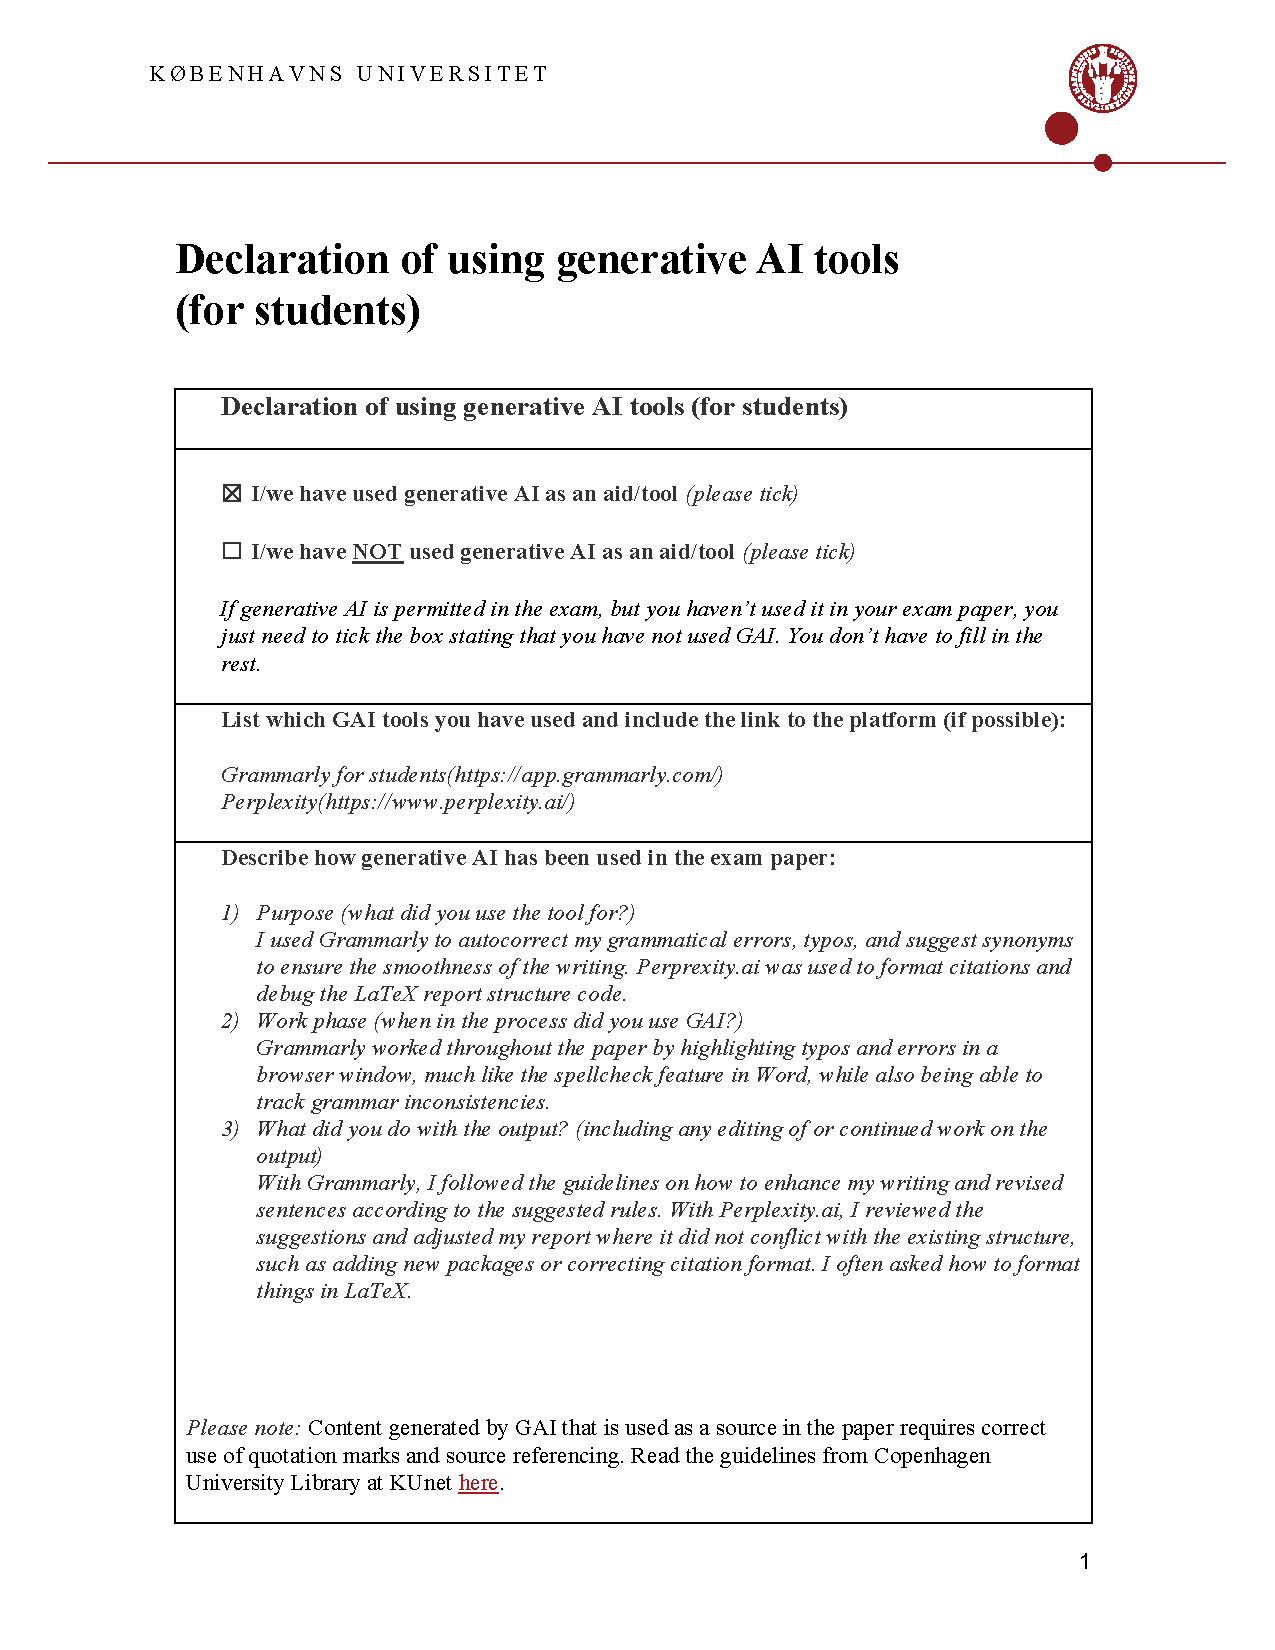
\includepdf[pages=-]{gai_declar.pdf}
\maketitle

\begin{abstract}
    \subfile{abstract}
\end{abstract}


{\small
\tableofcontents
}

\subfile{introduction}
\subfile{data}
% \subfile{theory}
\subfile{methodology}
\subfile{implementation}
\subfile{results}
\subfile{discussion}
\subfile{conclusion}

% \bibliographystyle{plainnat}
\printbibliography

\begin{appendices}
\subfile{appendix}
\end{appendices}

\end{document}
